\chapter{Regulator DMC}
\label{zad5}


\section{Algorytm działania}
Algorytm działania regulatora oraz implementacja została dobrze udokumentowana w pliku \verb+DMC.m +. Listing jego częsci algorytmicznej przedstawiony jest poniżej:
\begin{lstlisting}[style=custommatlab,frame=single,label={zad4_sim_lst},caption={Implementacja regulatora DMC},captionpos=b]

\end{lstlisting}


\section{Strojenie regulatora DMC}


Strojenie regulatora przeprowadzone zostało metodą automatyczną przy użyciu\\ funkcji \verb+ga(@DMC,nvars,[],[],[],[],lb,ub,[],IntCon,options)+. Strojonymi parametrami były $N$, $N_u$ oraz $\lambda$. Za dolne ograniczenie przyjęte zostały wartości $N=1$, $N_u = 1$, $\lambda = 1$, natomiast za górne $N=D$, $N_u = D$ oraz $\lambda = 1000$, gdzie $D = 116$. Wyniki strojenia regulatora przedstiowone są na wykresie \ref{fig:strojenie}.

\begin{figure}[h!]
	\centering
	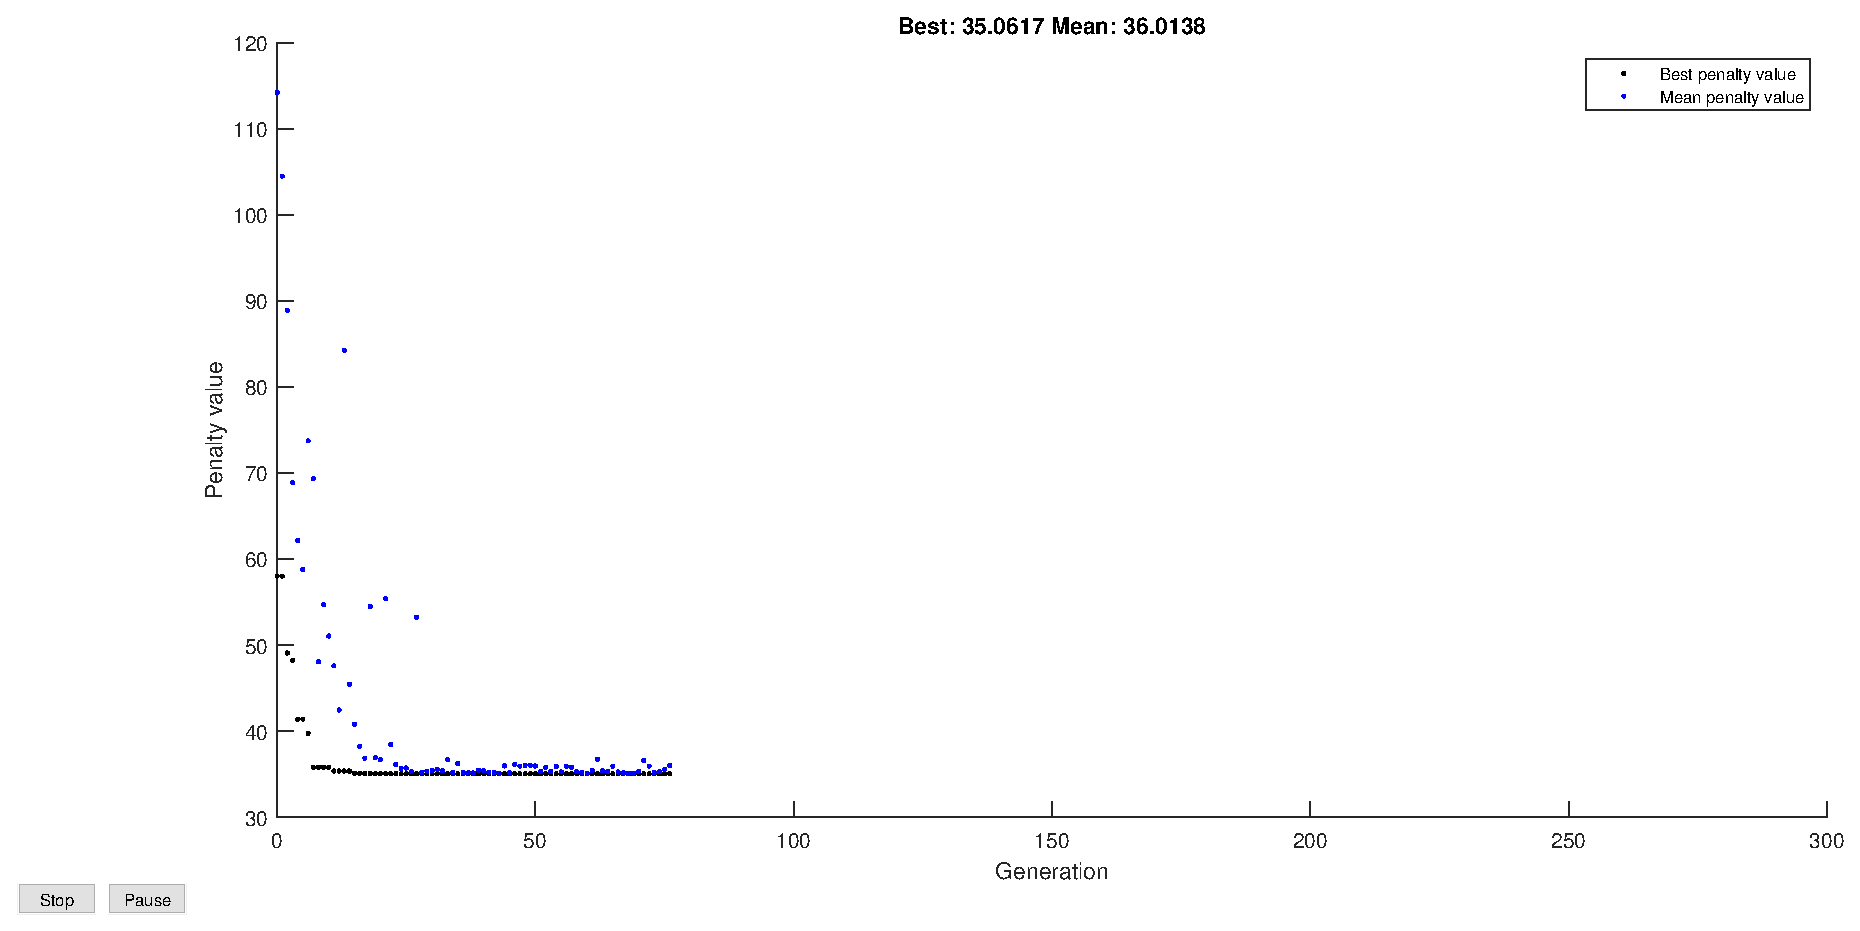
\includegraphics[scale=0.5]{Rys/strojenie.eps}
	\caption{Wyniki strojenia regulatora przy użyciu funkcji $ga$}
	\label{fig:strojenie}
\end{figure}

Przykładowy przebieg pokazujący pracę wystrojonego już regulatora można zobaczyć na wykresie \ref{fig:przebieg1}

\begin{figure}
	\centering
	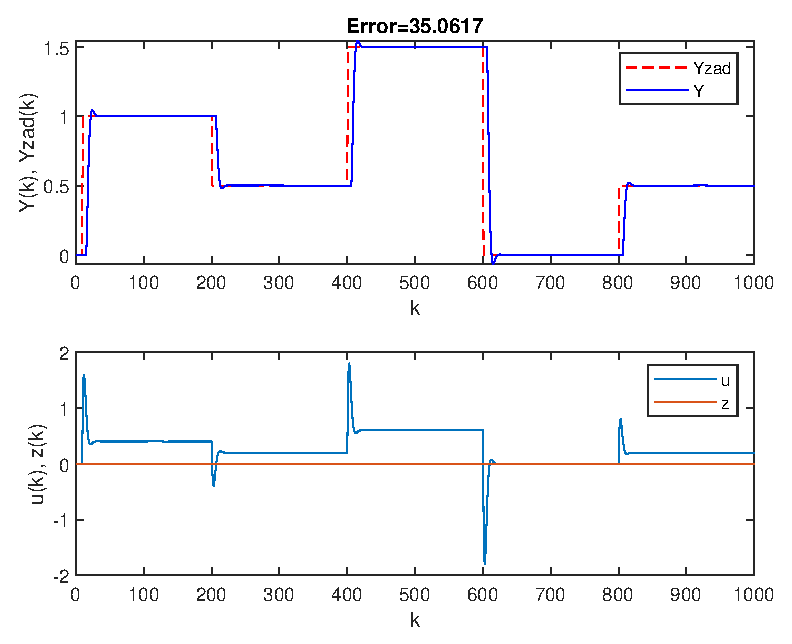
\includegraphics[scale=1]{Rys/przebieg1.eps}
	\caption{Przebieg dla parametrów $N = 116$, $N_u = 4$, $\lambda = 1$}
	\label{fig:przebieg1}
\end{figure}

\section{Obserwacje i wnioski}

Automatycznie dostrojony DMC okazał się lepszy (zgodnie z przewidywaniami), jednak interesujący jest fakt, iż otrzymano dwa tak samo dobre regulatory dla zupełnie różnych horyzontów sterowania i predykcji. Wynika z tego, że tak naprawdę jedyny parametr, która znacząco (oczywiscie poza bardzo krótkimi horyzontami predykcji) jest wartosć kary za sterowanie $\lambda$.
